% diagram_flow.tex — TikZ standalone template for a flow / pipeline diagram.
%
% Build with the bundled helper:
%   bash scripts/tikz_build.sh examples/diagram_flow.tex figures
% Or manually:
%   pdflatex -interaction=nonstopmode diagram_flow.tex
%   pdftoppm -r 300 -png diagram_flow.pdf diagram_flow
%
% Output is `standalone` — a tightly cropped vector PDF you can \includegraphics{}
% straight into a paper, OR rasterize to PNG for the render-view-fix loop.
%
% Palette: Okabe–Ito (colorblind-safe). Matches scripts/colors.py.

\documentclass[tikz,border=4pt]{standalone}
\usepackage{tikz}
\usepackage{helvet}
\renewcommand{\familydefault}{\sfdefault}
\usetikzlibrary{arrows.meta,positioning,shapes.geometric,calc,backgrounds,fit}

% --- Okabe–Ito colorblind-safe palette ----------------------------------------
\definecolor{okBlue}{HTML}{0072B2}
\definecolor{okOrange}{HTML}{E69F00}
\definecolor{okGreen}{HTML}{009E73}
\definecolor{okSky}{HTML}{56B4E9}
\definecolor{okVerm}{HTML}{D55E00}
\definecolor{okPurple}{HTML}{CC79A7}
\definecolor{okYellow}{HTML}{F0E442}
\definecolor{inkBlack}{HTML}{1A1A1A}

\begin{document}
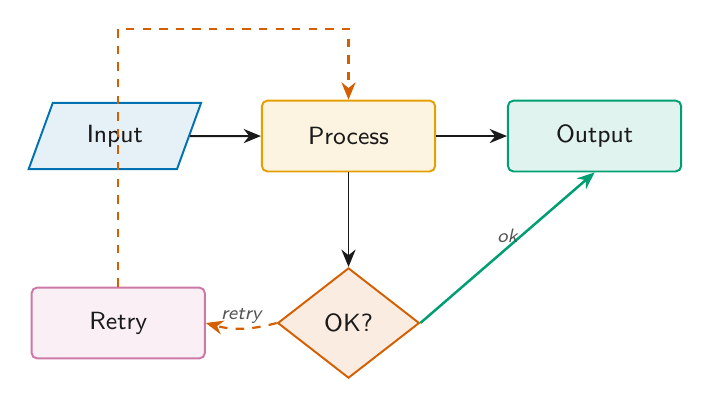
\begin{tikzpicture}[
  font=\small,
  >={Stealth[length=2.2mm,width=1.8mm]},
  line width=0.7pt,
  node distance=10mm and 9mm,
  every node/.style={inner sep=3pt},
  % --- Reusable styles -------------------------------------------------------
  stage/.style={                 % rounded process box, color via #1
    rectangle, rounded corners=2pt,
    draw=#1, fill=#1!12, text=inkBlack,
    minimum width=22mm, minimum height=9mm, align=center,
  },
  decision/.style={              % branching diamond
    diamond, aspect=1.6,
    draw=okVerm, fill=okVerm!12, text=inkBlack,
    minimum width=18mm, minimum height=14mm, align=center, inner sep=1pt,
  },
  io/.style={                    % input/output (parallelogram)
    trapezium, trapezium left angle=70, trapezium right angle=110,
    draw=#1, fill=#1!10, text=inkBlack,
    minimum width=22mm, minimum height=8mm, align=center,
  },
  flow/.style={->, draw=inkBlack, line width=0.7pt},
  loopflow/.style={->, draw=okVerm, line width=0.8pt, dashed},
  pass/.style={->, draw=okGreen, line width=0.9pt},
  lbl/.style={font=\scriptsize\itshape, text=inkBlack!75, inner sep=1.5pt},
]

% --- Nodes -------------------------------------------------------------------
\node[io=okBlue]                            (a) {Input};
\node[stage=okOrange,    right=of a]        (b) {Process};
\node[stage=okGreen,     right=of b]        (c) {Output};
\node[decision,          below=12mm of b]   (d) {OK?};
\node[stage=okPurple,    left=of d]         (e) {Retry};

% --- Arrows ------------------------------------------------------------------
\draw[flow] (a) -- (b);
\draw[flow] (b) -- (c);
\draw[flow] (b) -- (d);
\draw[loopflow] (d.west) to[bend left=15]
  node[lbl,above,pos=0.5]{retry} (e.east);
\draw[pass] (d.east) -- node[lbl,above]{ok} (c.south);

% --- Loop back: e -> b, routed above the top row to clear all nodes ----------
\coordinate (loopAnchor) at ($(b.north)+(0,9mm)$);
\coordinate (loopL)      at (e.north |- loopAnchor);
\coordinate (loopR)      at (b.north |- loopAnchor);
\draw[loopflow] (e.north) -- (loopL) -- (loopR) -- (b.north);

\end{tikzpicture}
\end{document}
